\documentclass[a4paper]{beamer}
%
% Josef Hlavac & Tomas Zahradnicky (21.10.2010)
%
%\usepackage{pgfpages}
%\pgfpagesuselayout{4 on 1}[a4paper,border shrink=5mm,landscape]
%\pgfpagesuselayout{resize}[a4paper,border shrink=5mm,landscape]
%\usepackage[czech]{babel}
\usepackage[utf8]{inputenc}
\usepackage{color}
\usetheme{Boadilla}
\useinnertheme{circles}
\usepackage{subfigure}
\usepackage[czech,slovak,english]{babel}%\useinnertheme{rounded}
%\useinnertheme{rectangles}
%\useinnertheme{balls}
%
%%%%%%%%%%%%%%%%%%%%%%%%%%%%%%%%%%%%%%%%%%%%%%%%%%%%%%%%%%%%%%%%%%
\newcommand\FirstName{Tomáš}
\newcommand\FirstNameAbbreviated{T}
\newcommand\LastName{Fedor}
\newcommand\Email{fedortom@fit.cvut.cz}
\newcommand\Faculty{Fakulta Informačních Technologií}
\newcommand\University{České vysoké učení technické v Praze}
\newcommand\FacultyAndUniversityAbbr{FIT ČVUT}

\author[\FirstNameAbbreviated. \LastName]{\FirstName{} \LastName}
\title[ARAP]{N-bodová deformácia obrazu využitím deformačného modelu ARAP}
\titlegraphic{
\includegraphics[width=1.5cm]{pic/LogoCVUT.pdf}}
\institute[\FacultyAndUniversityAbbr]{\\ \Faculty\\ \University}
\date{\today}
%
\begin{document}

\begin{frame}
	\titlepage
\end{frame}

\section*{Obsah}
	\begin{frame}[allowframebreaks]
		\frametitle{Obsah}
	\tableofcontents
\end{frame}

\section{Algoritmus}

\subsection{Program}
\begin{frame}	
	\frametitle{Program}
	\begin{itemize}
		\item Definovanie mriežky
		\item Opakuj:
		\begin{itemize}
			\item Nastavenie cieľovej polohy
			\item Regularizácia mriežky
			\item Prekreslenie obrázku
		\end{itemize}
	\end{itemize}
\end{frame}

\subsection{Embedding Lattice}
\begin{frame}	
	\frametitle{Embedding Lattice}
	\begin{itemize}
		\item nájdenie obsahu
		\item prekrytie maticou
		\begin{itemize}
			\item prepojené štvorce
			\item každý štvorec drží informáciu o pôvodnom stave
		\end{itemize}
		\item kontrolné body sa mapujú na vrcholy matice

		\begin{figure}
			\centering
			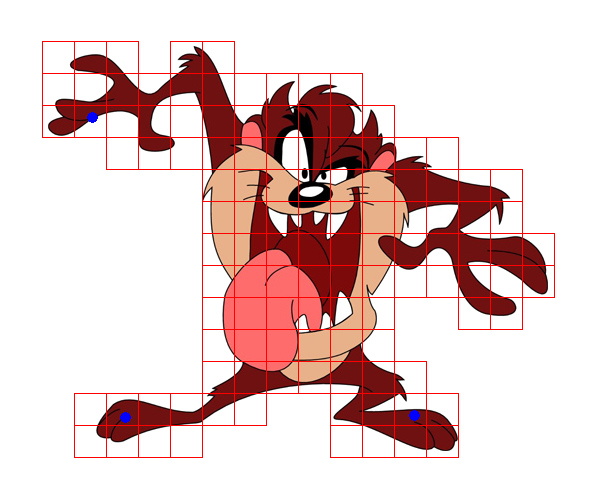
\includegraphics[height=0.5\textheight,keepaspectratio]{pic/taz_initial.jpg}
		\end{figure}
	\end{itemize}
\end{frame}

\subsection{Regularizácia}
\begin{frame}
	\frametitle{Regularizácia}
	\begin{itemize}
		\item zabezpečuje ARAP deformáciu
		\item minimalizácia vzdialenosti pôvodného štvorca k novému tvaru
		
		\begin{block}{Optimálna rotácia}
			\begin{displaymath}
		 		\mathbf{R^*} = \frac{1}{\mu}
		 		 \sum_i\left( 
					\begin{array}{c}
      					\mathbf{\hat{p}}_i \\
      					\mathbf{\hat{p}}^\bot_i
    				\end{array}
		 		 \right)
		 		 \left(
					\mathbf{\hat{q}}^T_i \, \mathbf{\hat{q}}^{\bot T}_i
		 		 \right)
		 	\end{displaymath}

		 	\begin{displaymath}
		 		\mathbf{\mu} = \sqrt{
		 			\left(\sum_i\
		 				\mathbf{\hat{q}}_i
		 				\mathbf{\hat{p}}^T_i
		 			\right)^2
		 			+
		 			\left(\sum_i\
		 				\mathbf{\hat{q}}_i
		 				\mathbf{\hat{p}}^{\bot T}_i
		 			\right)^2
		 		}
		 	\end{displaymath}

		 	\(\bot\) značí kolmý vektor
	 	\end{block}
	 	
	 	\begin{block}{Optimálna translácia}
	 		\begin{displaymath}
		 		\mathbf{t^*}^T = \mathbf{p}^T_c - \mathbf{R^*} \cdot \mathbf{q}^T_c
		 	\end{displaymath}
	 	\end{block}

	\end{itemize}
\end{frame}

\begin{frame}	
	\frametitle{Regularizácia 2}
	\begin{itemize}
		\item body matice sa spriemerujú
		\item iteratívne sa matica snaží dostať k cieľovej polohe
	\end{itemize}

	\begin{figure}
		\centering
		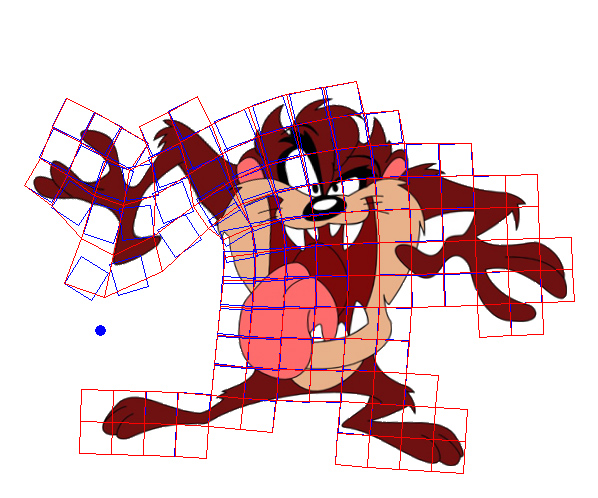
\includegraphics[height=0.5\textheight,keepaspectratio]{pic/taz_rigid.jpg}
		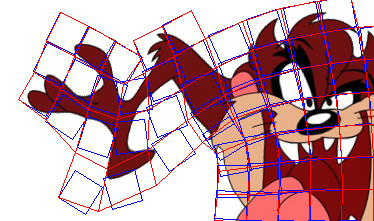
\includegraphics[height=0.5\textheight,keepaspectratio]{pic/taz_rigid_detail.jpg}
	\end{figure}
\end{frame}

\begin{frame}	
	\frametitle{Regularizácia 3}
	\begin{itemize}
		\item po odstránení kontrolných bodov sa vráti do pôvodnej polohy až na globálnu rotáciu a posun
	\end{itemize}

	\begin{figure}
		\centering
		
\includegraphics[height=0.5\textheight,keepaspectratio]{pic/taz_moved.jpg}
		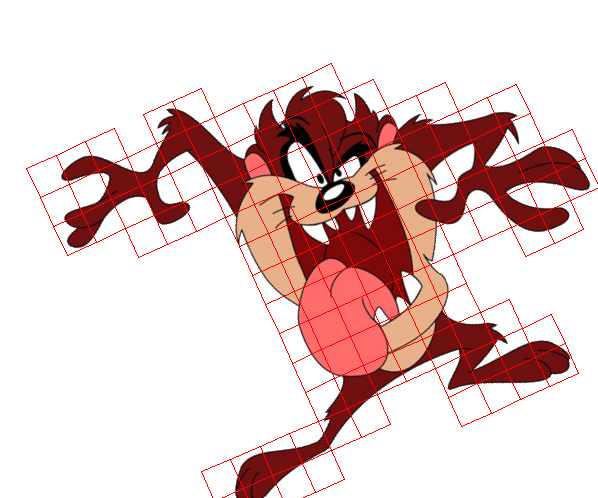
\includegraphics[height=0.5\textheight,keepaspectratio]{pic/taz_back.jpg}
	\end{figure}
\end{frame}

\subsection{Prekreslenie}
\begin{frame}
	\frametitle{Prekreslenie obrázku}
	\begin{itemize}
		\item homografia pre každý štvorec nového tvaru
		\item inverzná homografia
		\item najbližší pixel vs. bilineárna interpolácia
	\end{itemize}

	\begin{figure}
		\centering
		
\includegraphics[width=0.5\textwidth,keepaspectratio]{pic/taz_round.jpg}
		
\includegraphics[width=0.5\textwidth,keepaspectratio]{pic/taz_bilin.jpg}
	\end{figure}
\end{frame}

\section{Implementácia}
\begin{frame}
	\frametitle{Implementácia}
	\begin{itemize}
		\item Python
		\begin{itemize}
			\item TkInter - GUI
			\item numpy - matematika
		\end{itemize}
		\item C - pre výpočetne zložité časti
	\end{itemize}
\end{frame}

\section{Príklady}

\subsection{Krtek}
\begin{frame}
	\frametitle{Krtek}
	\begin{figure}
		\centering
		
\includegraphics[width=0.5\textwidth,keepaspectratio]{pic/results/krtek1}
		
\includegraphics[width=0.5\textwidth,keepaspectratio]{pic/results/krtek2}
	\end{figure}
\end{frame}

\subsection{Calvin \& Hobbes}
\begin{frame}
	\frametitle{Calvin \& Hobbes 1}
	\begin{figure}
		\centering
		
\includegraphics[width=0.5\textwidth,keepaspectratio]{pic/results/calvin1}
		
\includegraphics[width=0.5\textwidth,keepaspectratio]{pic/results/calvin2}
	\end{figure}
\end{frame}

\begin{frame}
	\frametitle{Calvin \& Hobbes 2}
	\begin{figure}
		\centering
		
\includegraphics[width=0.5\textwidth,keepaspectratio]{pic/results/calvin-hobbes1}
		
\includegraphics[width=0.5\textwidth,keepaspectratio]{pic/results/calvin-hobbes2}
	\end{figure}
\end{frame}

\subsection{Ratatouille}
\begin{frame}
	\frametitle{Ratatouille}
	\begin{figure}
		\centering
		
\includegraphics[width=0.5\textwidth,keepaspectratio]{pic/results/ratatouille1}
		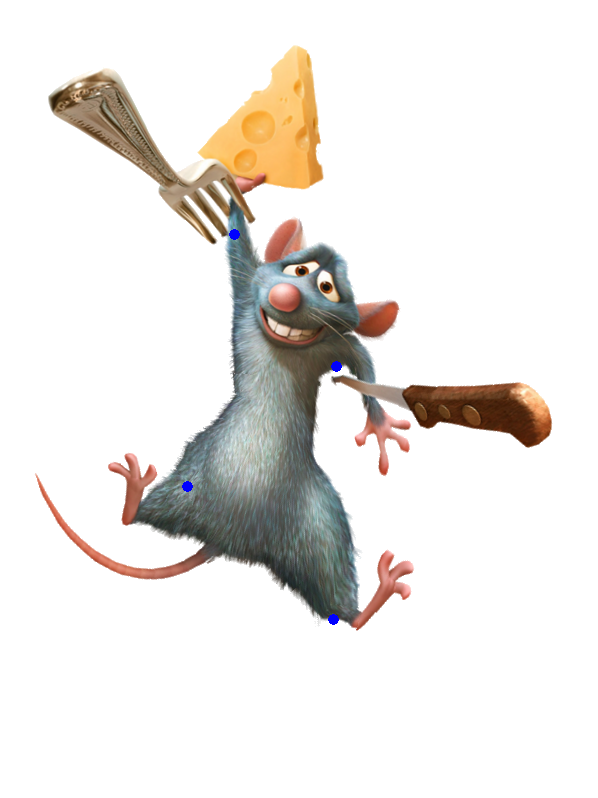
\includegraphics[width=0.5\textwidth,keepaspectratio]{pic/results/ratatouille2}
	\end{figure}
\end{frame}

\begin{frame}
	\vspace*{\fill}
	\begin{center}
		\Large Ďakujem za pozornosť
	\end{center}
	\vfill
\end{frame}

\end{document}

